\section{Physical application and finite-sampling experiments}\label{sec:physical}
We use open transverse-field Ising chains,
$H=-\sum_{i=1}^N X_i-J\sum_{i=1}^{N-1}Z_iZ_{i+1}$,
with initial state $\ket+^{\otimes N}$. Ising filtering is an established
benchmark \cite{QETU}; the application name is not a novelty claim.
The six cases have $N\in\{4,6,8\}$ and
$v=(N-1)J\in\{0.4,0.8\}$, so $J$ is not fixed as size changes.

\paragraph{Analytic input promises, before diagonalization.}
Let $\Delta=2-v$, $t^2=v^2/(N-1)$ and $d=t^2/\Delta$.
The unperturbed product state has energy $-N$, its orthogonal block
obeys $QHQ\succeq(-N+\Delta)Q$, and
$\|QV\ket+^{\otimes N}\|^2=t^2$: different bonds flip different pairs
in the $X$ basis. For a ground state $c\ket+^{\otimes N}+q$,
the variational bound $E_0\leq-N$ and the orthogonal block equation give
\[
 q=-(QHQ-E_0)^{-1}QV\ket+^{\otimes N}c,\quad
 -N-E_0\leq t^2/\Delta,\quad \|q\|\leq(t/\Delta)|c|.
\]
Thus $L=-N-d\leq E_0\leq U=-N$ and
$a=1/(1+t^2/\Delta^2)$ is a valid overlap lower bound.
With $R=N+v$, set $G=(H-LI)/(R-L)$, $u=d/(R-L)$ and $E=u/8$.
The physical tolerance is $d/8$, four times smaller than the prior
midpoint's worst error $d/2$. No true spectrum enters these promises.
Diagonalization is performed only after selection, to audit the result.
This promise derivation uses the known unperturbed gap; the weak-coupling
experiment is not evidence of an advantage specific to gap-free inputs.

\paragraph{Hamiltonian implementation convention.}
To apply the scalar theory to energy rather than a Gram minimum, assume
an ideal normalized Hermitian signal for $Y=2G-I$.
If $P(x)=\sum c_kT_k(2x-1)$ then
$F(y)=P((y+1)/2)=F_{\rm even}(y)+F_{\rm odd}(y)$.
Boundedness of $F$ implies boundedness of each parity part on $[-1,1]$.
Separate QSP realizations with margin $0.95$, Hermitian extraction and
LCU averaging give amplitude $0.475P(G)$. We include this factor of
one half in all nontrivial filtered application responses. The unfiltered
baseline omits extraction and has success probability one. Serial signal calls
are at most $4n$; preparation cost is the sensitivity choice $c_\psi=N$.
It is not a measured gate depth. Direct Pauli LCU for $Y$ has coefficient
norm $(2R+|R+L|)/(R-L)$, generally greater than one. The cost of realizing
the normalized signal from that LCU is not included. Consequently the
application compares an ideal oracle model, not physical gate resources.
A one-query Hadamard test on the controlled encoding of $Y$ has outcome
probability $(1+\langle Y\rangle)/2=\langle G\rangle$, supplying the
Bernoulli energy readout without assuming a free square-root Hamiltonian.

\paragraph{Application sanity check.}
At $N=4,v=0.8$, the initial energy bias is $0.053411$, above the tolerance
$0.022222$. The original selected degree-seven filter reduces the ideal
bias to $0.000368$. All six original application cases meet their bias
targets. Compared with selected guaranteed costs, the tested Chebyshev
cost factors are $1.001$--$1.173$; the three certified power cases have
factors $5.03$--$19.02$, and the other three lack a certified candidate
within the tested cap. These are finite parameter searches, not exhaustive
optimizations of the named families. Absolute costs remain large.
Saved original application phases have continuous amplitude error bounds
at most $2.04\times10^{-16}$. The following sampling study instead treats
the target polynomial itself as exact, as required by the ideal-circuit
assumption, and adds only finite measurement randomness.

\paragraph{Finite-budget catalog and reproducibility.}
For each physical prior, retain the original certified family candidates
and add LP candidates at biases
$b/u\in\{1/32,1/16,1/8,1/4,1/2\}$ and degrees
$n\in\{1,2,3,4,5,6,8,10,12,16\}$, with design/certificate margins
$0.98b,0.99b$. Failed continuous certificates are excluded.
Add the unfiltered mean and prior midpoint as baselines.
The six catalogs contain respectively $27,27,24,20,19,15$ responses
including the unfiltered mean; the midpoint is a separate option.
For each $B\in\{10^2,10^3,\ldots,10^9\}$ select by
\eqref{eq:finite-upper}--\eqref{eq:inverse-upper}, with abstention at
most $0.05$. All choices use priors only. There are 48 budget conditions;
21 select the prior midpoint. The rule changes degree and bias allocation
as the budget increases, rather than assuming the original expected-cost
choice is optimal for the new objective.

\begin{figure}[tb]
\centering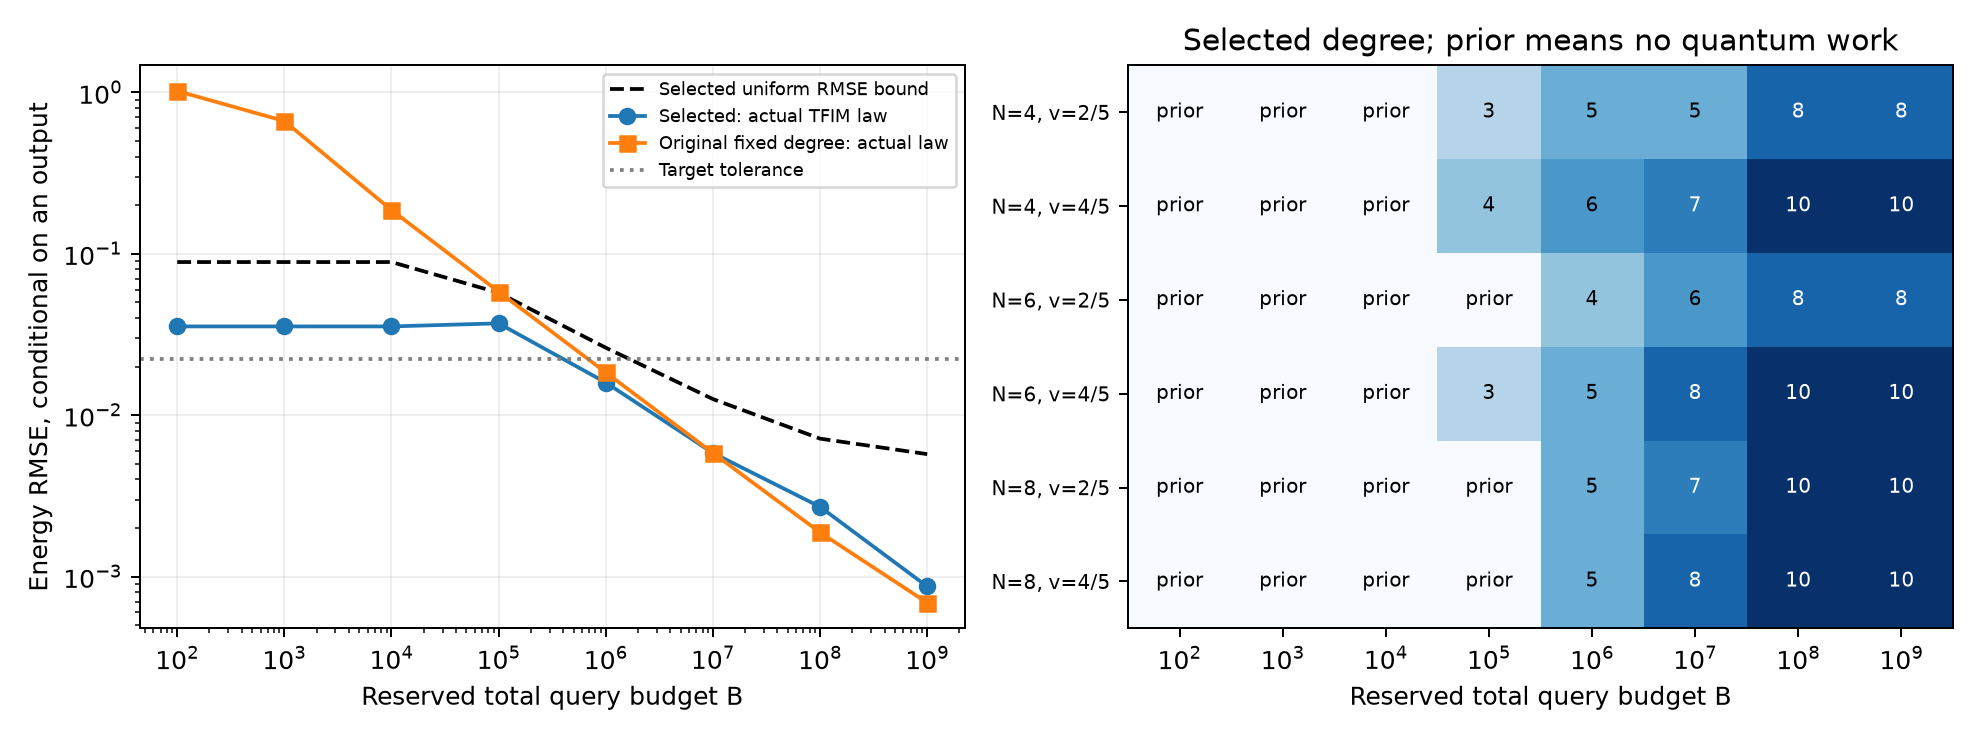
\includegraphics[width=\linewidth]{../../figures/finite_budget.png}
\caption{Ideal finite-budget selection. Left: four-spin $v=0.8$ case;
the black curve is a uniform RMSE bound, while colored curves are exact-law
numerical audits on that physical input. Right: selected degrees across
six priors; ``prior'' means no quantum work. A better uniform bound need
not give smaller actual risk on every individual spectrum.}
\label{fig:finite-budget}
\end{figure}

The three-energy reduction is checked independently on 100 random
21-energy inputs. Solving the moment LP preserves the conditional mean,
does not increase acceptance and does not decrease conditional MSE;
every reduced support has at most three energies. The largest observed
risk increase is $3.95$ times. This is a numerical check of a proved
reduction, not a certified global maximization over continuous spectra.

\paragraph{Finite counts, confidence and the bias floor.}
For the original degree-seven response at $N=4,v=0.8$:
\begin{center}\small
\begin{tabular}{rrrr}
\toprule
$B$ & conditional energy RMSE & no output & tolerance failure\\
\midrule
$10^2$ & $1.021$ & $0.711$ & $1.000$\\
$10^6$ & $0.01840$ & $<10^{-12}$ & $0.2265$\\
$10^7$ & $0.005830$ & $<10^{-12}$ & $0.000157$\\
\bottomrule
\end{tabular}
\end{center}
At $10^6$ query units the RMSE is below $0.022222$, yet the probability
of missing that tolerance is about $22.65\%$. Reporting RMSE alone would
therefore not justify a $95\%$ confidence statement. The probabilities
come from the binomial mixture \eqref{eq:finite-failure}, evaluated
numerically with omitted count mass approximately $10^{-12}$ or less.
They are not normal approximations or rational interval certificates.

Holding three filters fixed and varying $T=10^0,\ldots,10^{12}$ shows
the sampling regime and its transition to distinct bias floors.
The degree-four, seven and ten physical energy floors are respectively
$0.000763$, $0.000368$ and $0.000157$. Increasing shots cannot remove
those floors without changing the response.
Across 114 independent simulation batches we used 20,000 independent aggregate
binomial replicates each, or 2,280,000 total. Empirical MSEs agree with
the exact-law numerical predictions, with a largest discrepancy of
$3.31$ Monte Carlo standard errors. Replacing the random accepted count
by its mean in the budget study changes the predicted MSE by factors
ranging from $0.280$ to $1.293$ in these tests.
Exact rational enumeration and arithmetic controls supply 183 additional
checks; they are distinct from the Monte Carlo consistency study.

\begin{figure}[tb]
\centering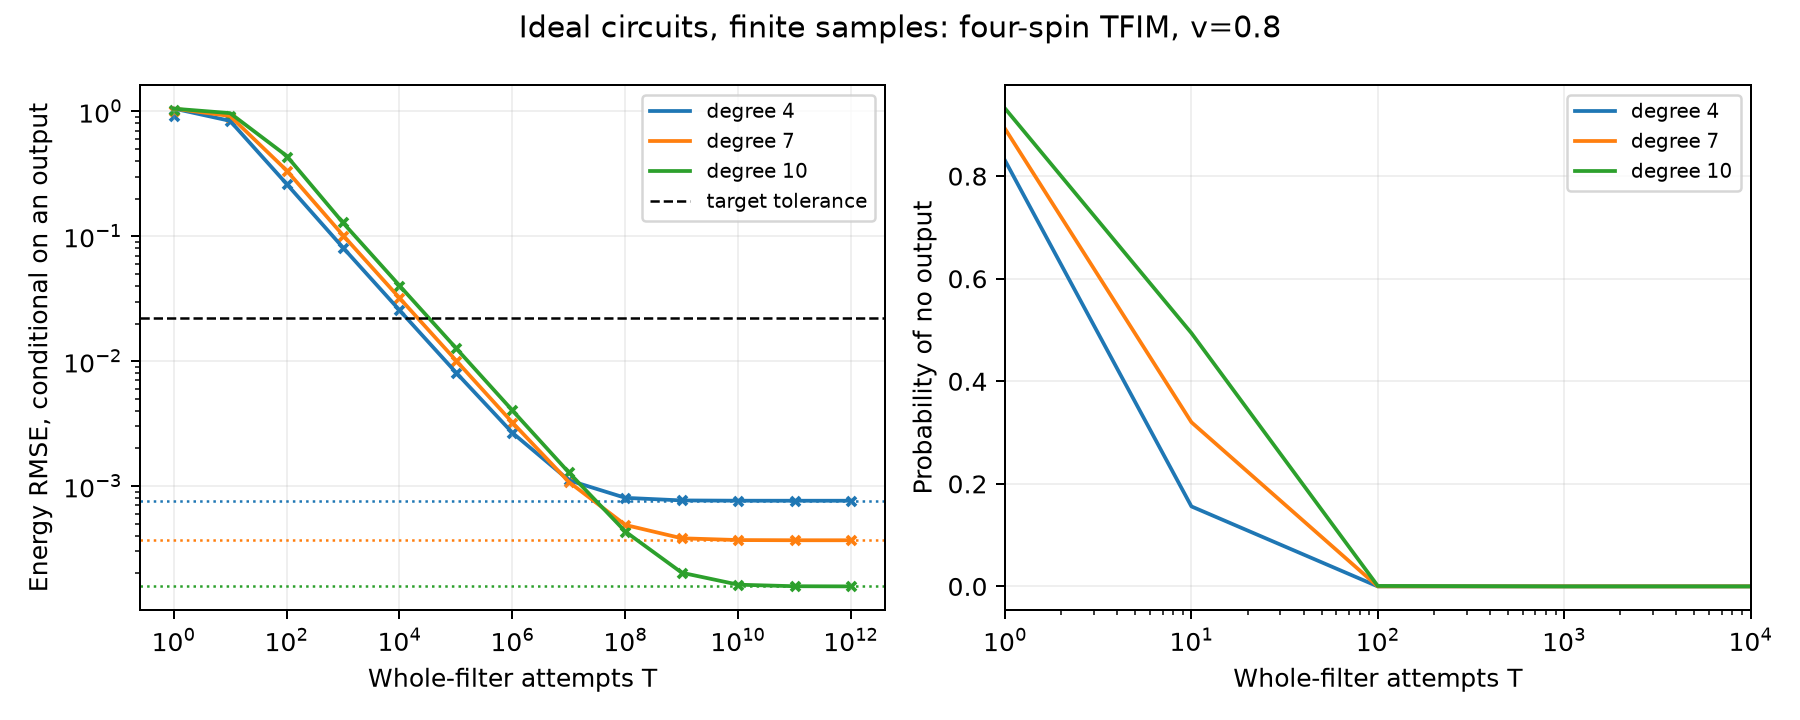
\includegraphics[width=\linewidth]{../../figures/finite_precision.png}
\caption{Ideal circuits with finite sampling on the four-spin $v=0.8$
input. Lines: exact-law numerical RMSE; crosses: Monte Carlo;
dotted levels: bias floors. Right: probability of no accepted sample.
The dashed target is a tolerance, not a confidence bound.}
\label{fig:finite-precision}
\end{figure}

The finite-budget selection is intentionally conservative. For example,
at $B=10^8$ in the representative case it selects degree ten, whose
actual RMSE is $0.00270$, while the original degree seven has $0.00188$.
The former minimizes the computed \emph{uniform bound} in the catalog;
it is not an instance-wise optimum. These small, classically tractable
Ising chains do not establish quantum advantage, thermodynamic scaling,
or superiority to QET-U or other estimators. What the extension adds is
an explicit finite-attempt accuracy/abstention objective, its spectral
reduction and an end-to-end reproducible ideal sampling test.
